\documentclass[12pt, a4paper]{exam}

\usepackage{graphicx}
\usepackage{listings}
\usepackage{xcolor}
\usepackage{multicol}

\definecolor{codegreen}{rgb}{0,0.6,0}
\definecolor{codegray}{rgb}{0.5,0.5,0.5}
\definecolor{codepurple}{rgb}{0.58,0,0.82}
\definecolor{backcolour}{rgb}{0.95,0.95,0.92}

\lstdefinestyle{mystyle}{
    backgroundcolor=\color{backcolour},   
    commentstyle=\color{codegreen},
    keywordstyle=\color{magenta},
    numberstyle=\tiny\color{codegray},
    stringstyle=\color{codepurple},
    basicstyle=\ttfamily\footnotesize,
    breakatwhitespace=false,         
    breaklines=true,                 
    captionpos=b,                    
    keepspaces=true,                 
    numbers=left,                    
    numbersep=5pt,                  
    showspaces=false,                
    showstringspaces=false,
    showtabs=false,                  
    tabsize=2
}

\lstset{style=mystyle}

\begin{document}

\begin{center}
\Large BTS CIEL2 — Évaluation langage C++ et MQTT
\end{center}
\begin{center}
11/02/2026 \hfill Nom et prénom:\enspace \hrulefill
\end{center}

\pointsinrightmargin

\begin{questions}

\question{Cochez la bonne réponse :}

\begin{parts}

\part[1] Quelle définition convient le mieux à la notion de constructeur (en langage C++) :
\begin{checkboxes}
 \choice Le constructeur simplifie la construction de classes complexes
 \choice Le constructeur est uniquement appelé quand on utilise le mot clé \texttt{new}
 \CorrectChoice Le constructeur est automatiquement appelé lors de la création d'une instance d'une classe
\end{checkboxes}

\part[1] Quelle est la différence entre \texttt{malloc} et \texttt{new} :
\begin{checkboxes}
 \choice \texttt{malloc} initialise la mémoire avec des 0, \texttt{new} ne fait rien ce qui est plus performant 
 \CorrectChoice \texttt{malloc} alloue de la mémoire brute sans appeler de constructeur
 \choice  il n'y en a pas, c'est simplement que \texttt{new} et \texttt{delete} sont plus mnémotechniques
\end{checkboxes}

\part[1] Laquelle de ces lignes n'est pas correcte :
\begin{checkboxes}
 \choice \texttt{CryptoMonster * my\_monster;}
 \choice \texttt{CryptoMonster my\_monster("I'm a crypto monster");}
 \CorrectChoice \texttt{CryptoMonster my\_monster = new CryptoMonster("I'm a crypto monster");}
\end{checkboxes}

\part[1] Le C++ introduit la notion de référence, quelle est sa principale différence avec un pointeur :
\begin{checkboxes}
 \CorrectChoice la référence ne peut pas être réassignée après son initialisation
 \choice le pointeur permet d'addresser n'importe quel type, la référence ne fonctionne qu'avec des types provenant du C++
 \choice le pointeur n'existe pas en C++, il faut utiliser la référence à la place 
\end{checkboxes}

\part[1] Quel type conteneur utiliseriez-vous pour stocker un nombre indéfini d'éléments :
\begin{checkboxes}
 \choice \texttt{std::array}
 \CorrectChoice \texttt{std::vector}
 \choice \texttt{std::growable\_array}
\end{checkboxes}

\part[1] Quelle est la signification du sigle RAII (dans l'univers C++):
\begin{checkboxes}
 \choice Resource Allocation Is Immediate 
 \CorrectChoice Resource Acquisition Is Initialization
 \choice Runtime Automatic Initialization Interface
\end{checkboxes}

\pagebreak

\part[1] Quelle est la différence la plus notable entre une classe (\texttt{class}) et une structure (\texttt{struct}) :
\begin{checkboxes}
 \CorrectChoice la classe privatise ses membres par défaut
 \choice la structure ne peut pas utiliser \texttt{this}
 \choice la structure ne peut pas avoir de méthodes
\end{checkboxes}

\part[1] Que signifie le sigle MQTT
\begin{checkboxes}
 \choice Message Queue Transfer Technology
 \CorrectChoice Message Queuing Telemetry Transport
 \choice Minimal Query Telemetry Transport
\end{checkboxes}

\part[1] Quelles sont les garanties du niveau 2 de QoS de MQTT
\begin{checkboxes} 
 \choice les messages venant de certains capteurs sont prioritaires
 \choice l'émetteur du message reçoit un acquittement pour valider la bonne réception
 \CorrectChoice le receveur reçoit exactement une fois le message
\end{checkboxes}

\part[1] Laquelle de ces affirmations est fausse concernant MQTT
\begin{checkboxes} 
 \choice MQTT s'appuie sur le protocole TCP de la couche 4 du modèle OSI  
 \choice Un client abonné peut recevoir deux fois le même message
 \CorrectChoice Tout le monde est client il n'y a pas de notion de serveur 
\end{checkboxes}

\end{parts}

\vspace{1em}
\question[5]{Dessinez le schéma d'une architecture MQTT mettant en œuvre un capteur de temperature et un afficheur.}
\noindent\textit{Remarque : faîtes bien attention au sens des flêches et mettez en avant le maximum d'informations concernant le protocole MQTT.}

\pagebreak

\question{Représentez l'état de la mémoire sur le schéma.}
\begin{parts}

\part[2.5]{Lorsque le programme a terminé la ligne 15.}
\begin{multicols}{2}
\begin{lstlisting}[language=C++]
struct Point {int x; int y;};

Point* new_point_from(Point a, Point b)
{
  Point* p = new Point();
  p->x = a.x + b.x;
  p->y = a.y + b.y;
  return p;
}

int main()
{
  Point a = {10, 10};
  Point b = {20, 20};
  Point* p = new_point_from(a, b);
  delete p;
}
\end{lstlisting}

\columnbreak

\centering
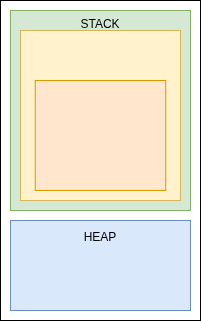
\includegraphics[]{stack.png}

\end{multicols}

\pagebreak

\part[2.5]{Lorsque le programme a terminé la ligne 17.}

\begin{multicols}{2}
\begin{lstlisting}[language=C++]
struct Point {int x; int y;};

Point* new_point_from(Point& a, Point& b)
{
  Point* p = new Point();

  p->x = a.x + b.x;
  p->y = a.y + b.y;

  return p;
}

int main()
{
  Point a = {10, 10};
  Point b = {20, 20};
  Point* p = new_point_from(a, b);
  delete p;
}
\end{lstlisting}

\columnbreak

\centering
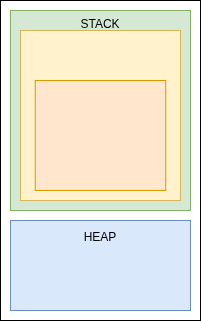
\includegraphics[]{stack.png}

\end{multicols}
\end{parts}

\end{questions}

\end{document}

